\documentclass[xcolor=dvipsnames]{beamer}
% \documentclass[aspectratio=169,xcolor=dvipsnames]{beamer}
\usepackage{ods}
\usepackage{ods-figs}
\usepackage[cm]{sfmath}
\usepackage{xmpmulti}
\usepackage{amssymb}
%\usepackage{enumitem}

% \setlength{parskip}{3pt}

\newcommand{\torso}[2]{#1\langle #2\rangle}
\DeclareMathOperator{\tw}{tw}

% \setbeamercovered{transparent}

% \setlength{\leftmargini}{0pt}

\newcommand{\N}{\mathbb{N}}
\DeclareMathOperator{\pth}{path}

\title[Adjacency Labelling]{Adjacency Labelling
  \newline for Proper Minor-Closed Graph Classes}
\author[Dujmović \textit{et al}]{Vida Dujmović, Cyril Gavoille, Gwenaël Joret, \newline Piotr Micek, Pat Morin, David Wood}

% START MACROS
\newcommand{\calA}{\mathcal{A}}
\newcommand{\calB}{\mathcal{B}}
\newcommand{\calC}{\mathcal{C}}
\newcommand{\calD}{\mathcal{D}}
\newcommand{\calE}{\mathcal{E}}
\newcommand{\calF}{\mathcal{F}}
\newcommand{\calG}{\mathcal{G}}
\newcommand{\calH}{\mathcal{H}}
\newcommand{\calI}{\mathcal{I}}
\newcommand{\calJ}{\mathcal{J}}
\newcommand{\calK}{\mathcal{K}}
\newcommand{\calL}{\mathcal{L}}
\newcommand{\calM}{\mathcal{M}}
\newcommand{\calN}{\mathcal{N}}
\newcommand{\calO}{\mathcal{O}}
\newcommand{\calP}{\mathcal{P}}
\newcommand{\calQ}{\mathcal{Q}}
\newcommand{\calR}{\mathcal{R}}
\newcommand{\calS}{\mathcal{S}}
\newcommand{\calT}{\mathcal{T}}
\newcommand{\calU}{\mathcal{U}}
\newcommand{\calV}{\mathcal{V}}
\newcommand{\calW}{\mathcal{W}}
\newcommand{\calX}{\mathcal{X}}
\newcommand{\calY}{\mathcal{Y}}
\newcommand{\calZ}{\mathcal{Z}}
% END MACROS
\begin{document}

\begin{frame}
  \titlepage
  \vspace{-1.9cm}
  \begin{tabular}{cc}
    \multicolumn{2}{c}{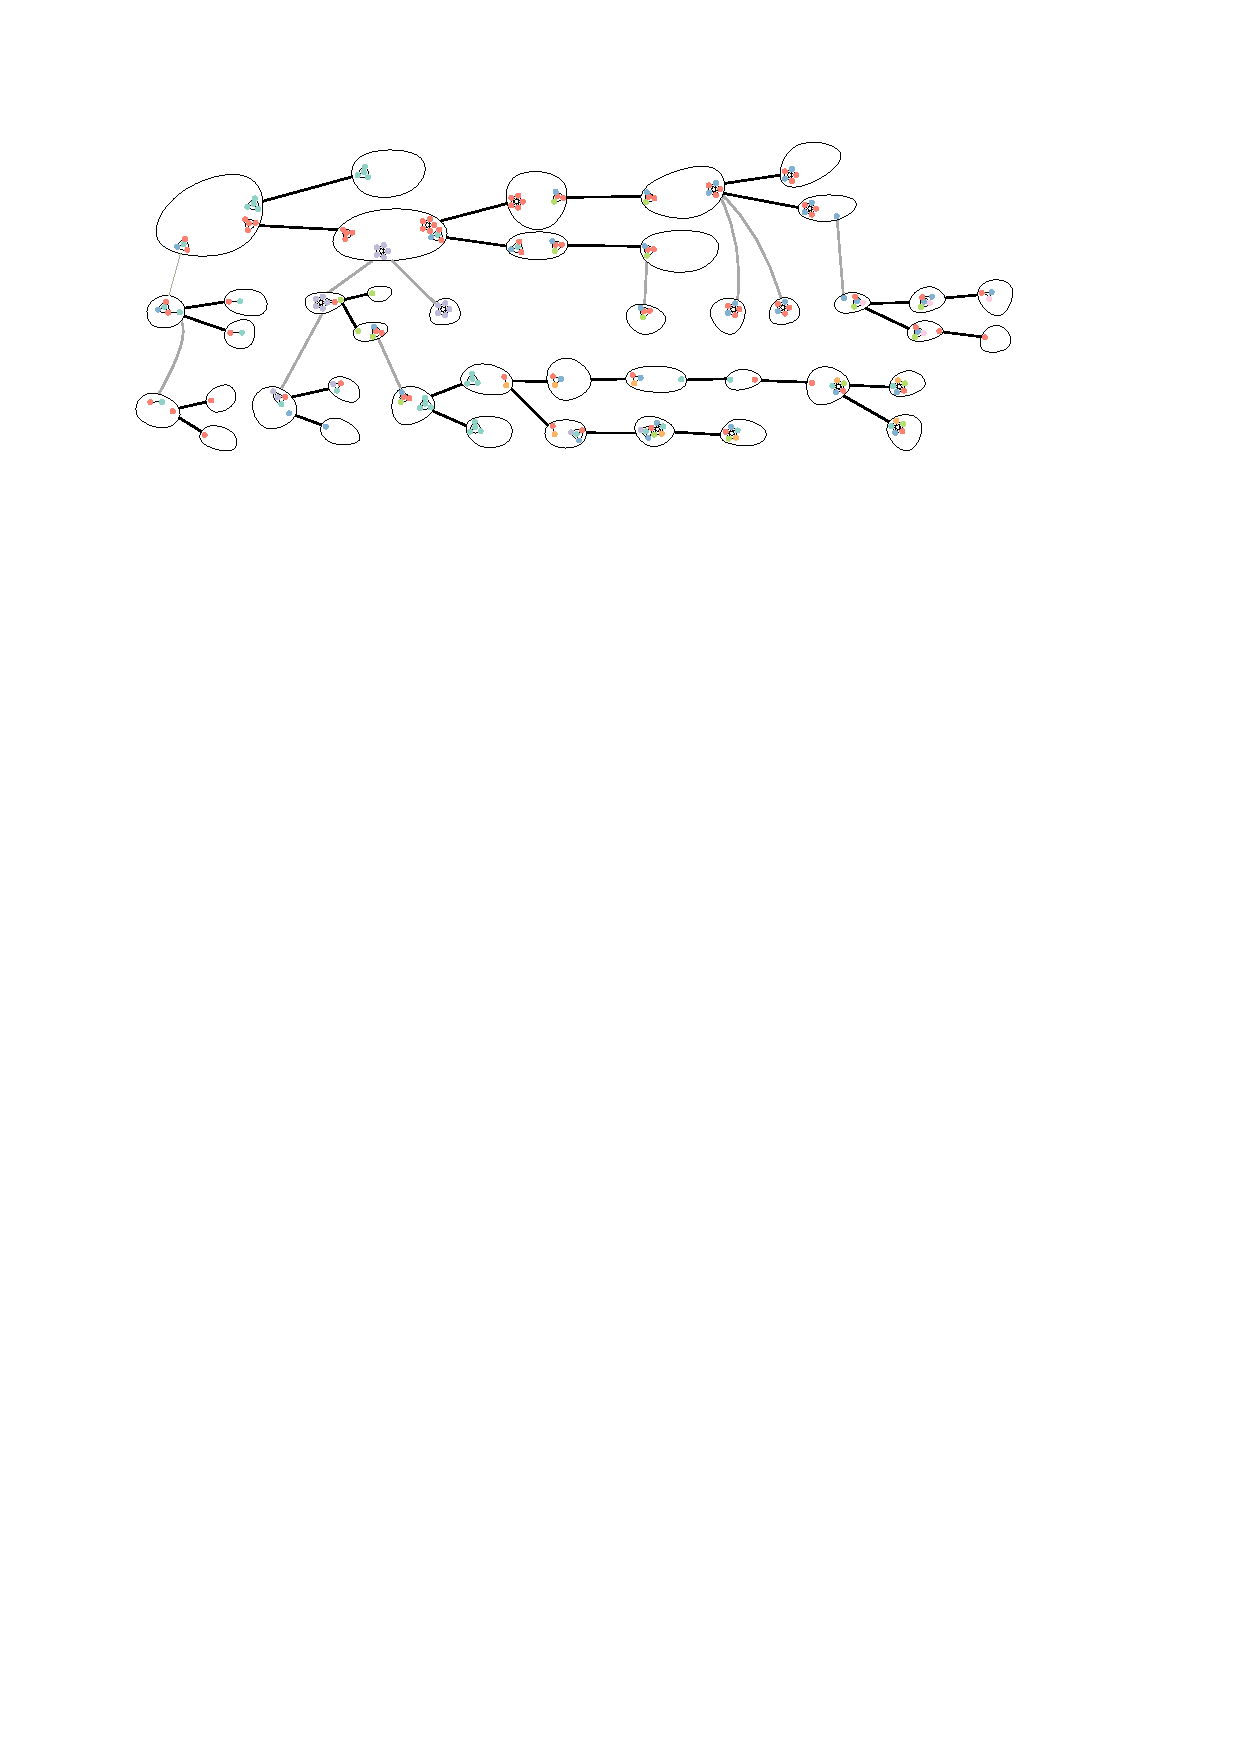
\includegraphics[page=1,width=.6\textwidth]{figs/t_tprime}} \\
    \includegraphics[page=3,width=.452\textwidth]{figs/t_tprime} &
    \includegraphics[page=6,width=.452\textwidth]{figs/t_tprime}
  \end{tabular}
\end{frame}

\begin{frame}
  \frametitle{A Problem as Old as Us?}

  \begin{center}
    \only<+>{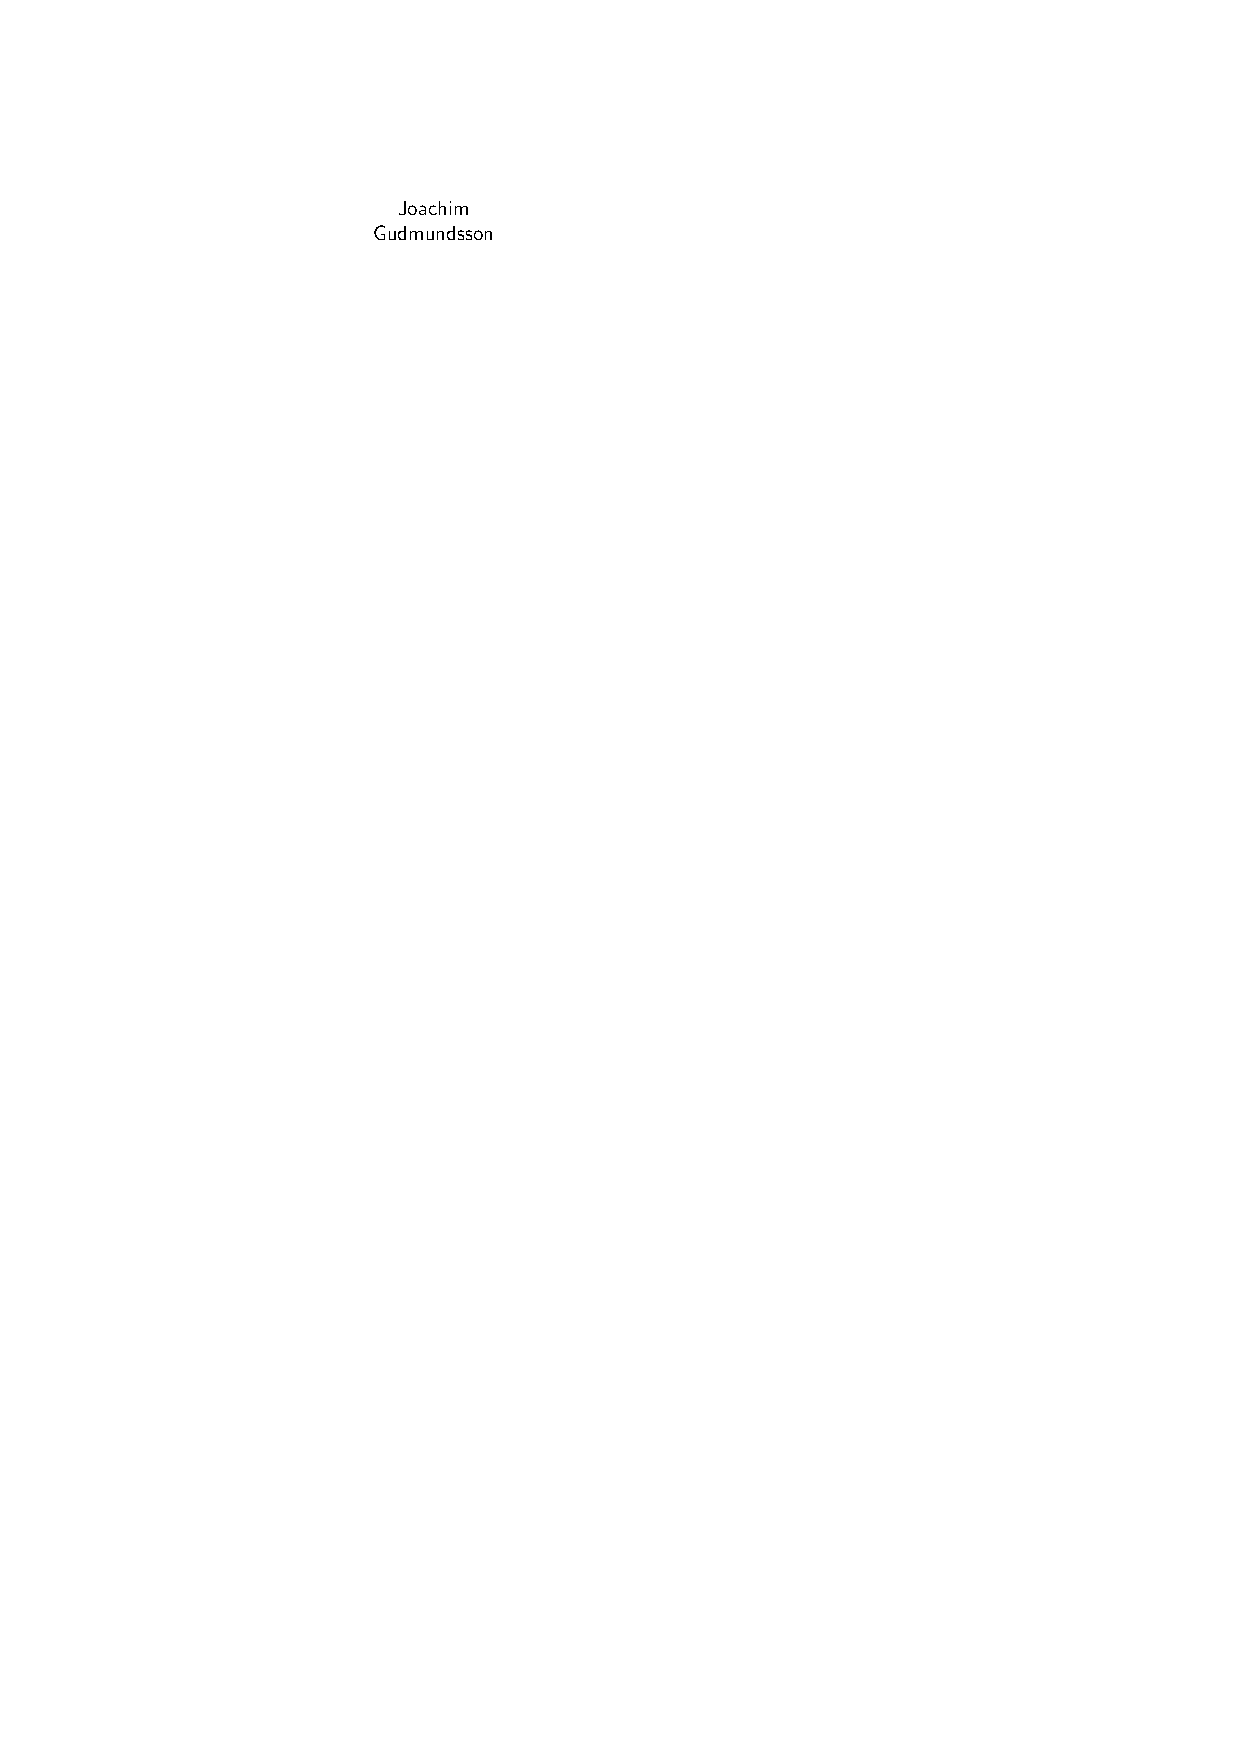
\includegraphics[page=1,width=.9\textwidth]{figs/names}}%
    \only<+>{\includegraphics[page=2,width=.9\textwidth]{figs/names}}%
    \only<+>{\includegraphics[page=3,width=.9\textwidth]{figs/names}}%
    \only<+>{\includegraphics[page=4,width=.9\textwidth]{figs/names}}%
    \only<+>{\includegraphics[page=2,width=.9\textwidth]{figs/names}}%
    \only<+->{\includegraphics[page=5,width=.9\textwidth]{figs/names}}%
  \end{center}
  \uncover<+>{Patronyms: the oldest naming system in human history(?)}
\end{frame}



\begin{frame}
  \frametitle{Adjacency Labelling}
  \framesubtitle{Labelling and Testing for a graph $G$}

  \begin{itemize}
    \item $A:\{0,1\}^*\times\{0,1\}^*\to \{0,1\}$ (\emph{adjacency tester})
    \item $\ell:V(G)\to\{0,1\}^*$ (\emph{labelling})
    \item $\ell$ is an \emph{adjacency labelling} of $G$ for $A$ if
        $
            A(\ell(v),\ell(w)) = \begin{cases}
                1 & \text{if $vw\in E(G)$} \\
                0 & \text{if $vw\not\in E(G)$}
        \end{cases}
        $\newline
        for each $v,w\in V(G)$,
    \end{itemize}
    \begin{center}
      \only<1>{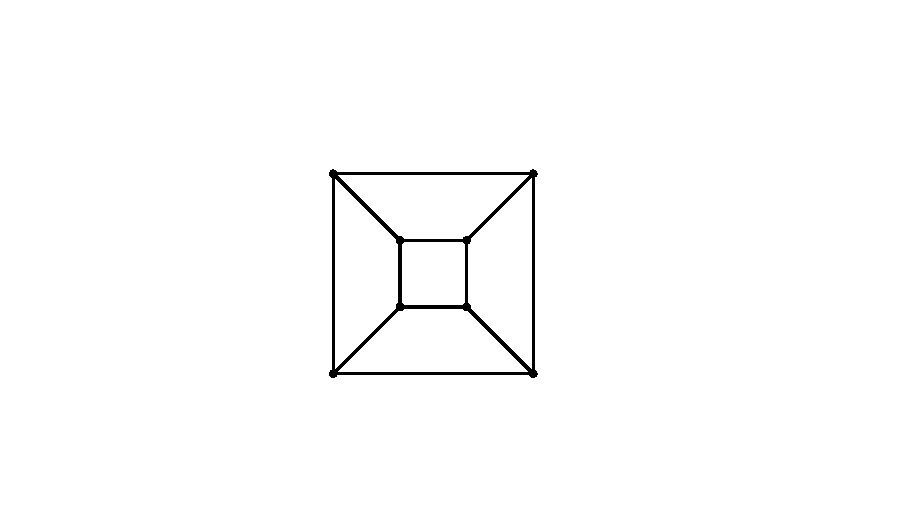
\includegraphics[page=1]{figs/labelling-scheme}}%
      \only<2>{\includegraphics[page=2]{figs/labelling-scheme}}%
      \only<3>{\includegraphics[page=3]{figs/labelling-scheme}}%
      \only<4>{\includegraphics[page=4]{figs/labelling-scheme}}%
    \end{center}
\end{frame}

\begin{frame}
    \frametitle{Adjacency Labelling}
    \framesubtitle{Labelling schemes for graph classes}

    \begin{itemize}
        \item<+->A graph class $\calG$ has an \emph{$f(n)$-bit labelling scheme} if \begin{itemize}
            \item there exists $A:\{0,1\}^*\times\{0,1\}^*\to\{0,1\}$ such that
            \item for each $n$-vertex $G\in\calG$ there exists an adjacency labelling $\ell:V(G)\to\{0,1\}^{f(n)}$ of $G$ for $A$
        \end{itemize}
    \end{itemize}
    \uncover<+->{Example: $\calG:=\{Q_d:d\in \mathbb{N}\}$ (hypercubes)}
    \begin{center}
      \only<1-2>{\includegraphics[page=8]{figs/labelling-scheme}}%
      \only<+>{\includegraphics[page=5]{figs/labelling-scheme}}%
      \only<+>{\includegraphics[page=6]{figs/labelling-scheme}}%
      \only<+>{\includegraphics[page=7]{figs/labelling-scheme}}%
    \end{center}
\end{frame}


\begin{frame}
    \frametitle{Universal Graphs}
    \framesubtitle{Labelling schemes and universal graphs}

    \begin{itemize}
        \item<+->\textbf{Theorem (Folklore):}  If a graph class $\calG$ has an $f(n)$-bit \emph{injective} labelling scheme then, for each $n\in\N$ there exists a graph $U_n$ such that
        \begin{itemize}
            \item $|V(U_n)|=2^{f(n)}$
            \item For each $n$-vertex $G\in\calG$, $G$ appears as an induced subgraph of $U_n$
        \end{itemize}
        \item<+->Proof: $V(U_n):=\{0,1\}^{f(n)}$, $E(U_n):=\{vw:A(v,w)=1\}$.
        \item<+->$U_n$ is called an \emph{(induced) universal} graph for $n$-vertex members of $\calG$.
    \end{itemize}
\end{frame}


\begin{frame}
    \frametitle{Previous Results}
    \framesubtitle{Trees and Bounded Treewidth Graphs}

    \begin{center}
        \begin{tabular}{@{}lll@{}} \hline
            \multicolumn{3}{|c|}{\textbf{Trees}} \\ \hline
            \boldmath $f(n)$ & \boldmath $|U_n|$ & \textbf{Reference}  \\ \hline
            {$\lceil 2\log n\rceil$} & $O(n^2)$ & Humanity \\
            & & (unique name + parent name)   \\\hline
            {$\log n+\log\log n+O(1)$} & $O(n\log n)$ & Chung (1990)   \\
            $\log n + O(\log^* n)$ & $n2^{O(\log^* n)}$ & Alstrup-Rauhe (2006) \\
            {$\log n + O(1)$} & $O(n)$ & Alstrup-Dahlgaard-Knudsen (2017) \\[2em] \hline
            \multicolumn{3}{|c|}{\textbf{Bounded treewidth graphs}} \\ \hline
            {$\log n + o(\log n)$} & $n^{1+o(1)}$ & Gavoille-Labourel (2007)
        \end{tabular}
    \end{center}
\end{frame}


\begin{frame}
    \frametitle{Planar Graphs}
    % \framesubtitle{Planar Graphs}
    \begin{center}
        \begin{tabular}{@{}lll@{}} \hline
            \multicolumn{3}{|c|}{\textbf{Planar graphs}} \\ \hline
            \boldmath $f(n)$ & \boldmath$|U_n|$ & \textbf{Reference} \\ \hline %& Techniques \\ \hline
            {$6\log n$} & $n^6$ & Muller (1988) \\ %& 5-degeneracy \\
            {$4\log n$} & $n^4$ & Kannan-Naor-Rudich (1988) \\ %& 3-orientation \\
            {$3\log n + O(1)$} & $O(n^3)$ & ---  \\ %& arboricity + trees \\
            {$2\log n + o(\log n)$} & $n^{2+o(1)}$ & Gavoille-Labourel (2007) \\ % \\ & 2-outerplanar decomp. \\
            {$\tfrac{4}{3}\log n + o(\log n)$} & $n^{\tfrac{4}{3}+o(1)}$ & Bonamy-Gavoille-Pilipczuk (2020) \\ %& product structure  \\
            {$\log n + o(\log n)$} & $n^{1+o(1)}$ & Dujmović-Esperet-Gavoille-\\ & & Joret-Micek-Morin (2021) %& product structure  \\
        \end{tabular}
    \end{center}
\end{frame}

\begin{frame}
    \frametitle{Planar Graphs}
    % \framesubtitle{Planar Graphs}
    \begin{center}
        \begin{tabular}{lll} \hline
          \multicolumn{3}{|c|}{\textbf{Planar graphs}} \\ \hline
            \boldmath$f(n)$ & \textbf{Ref} & \textbf{Techniques} \\ \hline
            {$6\log n$} & M88 & 5-degeneracy \\
            {$4\log n$} & KNR (1988) & 3-orientation \\
            {$3\log n + O(1)$} & --- & arboricity + trees \\
            {$2\log n + o(\log n)$} & GL07 & 2-outerplanar decomp. \\
            & & + treewidth \\
            {$\tfrac{4}{3}\log n + o(\log n)$} & BGP20 & product structure  \\
            {$\log n + o(\log n)$} & DEGJMM21 & product structure  \\
        \end{tabular}
    \end{center}
\end{frame}


\begin{frame}
  \frametitle{Planar graphs: $2\log n+o(\log n)$}

  \begin{center}
    \only<+>{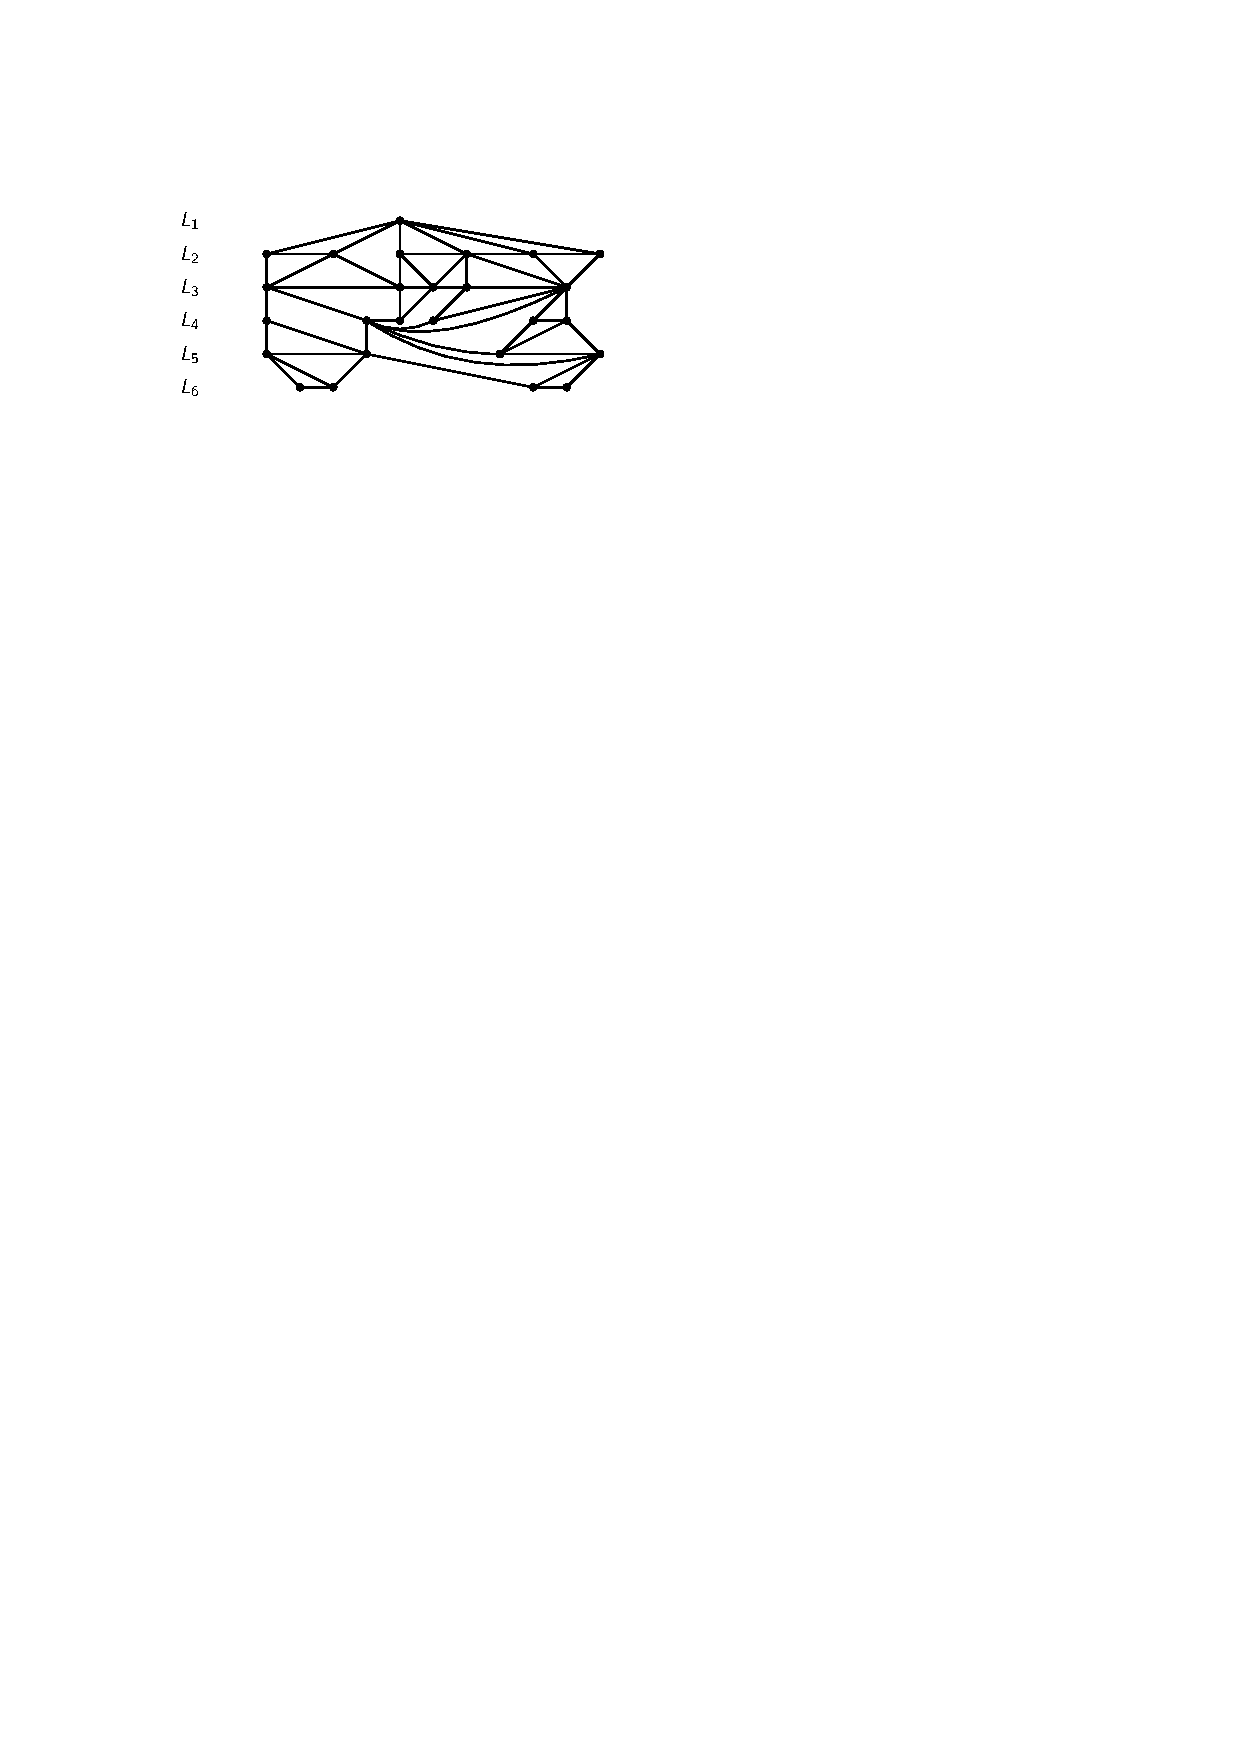
\includegraphics[page=1]{figs/planar}}%
    \only<+>{\includegraphics[page=2]{figs/planar}}%
    \only<+>{\includegraphics[page=3]{figs/planar}}%
    \only<+>{\includegraphics[page=4]{figs/planar}}%
    \only<+>{\includegraphics[page=5]{figs/planar}}%
  \end{center}
  \uncover<4->{$\ell_{G_1}$, $\ell_{G_2}$ and $A'$ come from Gavoille-Labourel 2007}
\end{frame}


\begin{frame}
  \frametitle{Planar graphs: $3\log n+o(\log n)$}

  \begin{itemize}
    \item BFS layering $L_1,L_2,\ldots,L_h$
    \item Labelling $\ell_{G_i}$ of $G_i=[L_i\cup L_{i+1}]$ (bounded treewidth)
    \item<+-> For $v\in L_i$, $\ell(v)=\langle i, \ell_{G_i}(v), \ell_{G_{i-1}}(v)\rangle$
    \item<+-> $|\ell(v)|\approx \log h + \log|V(G_i)|+\log|V(G_{i-1})|\approx 3\log n$
    \item<+->Adjacency testing: $\langle i,\ell_{G_i}(v),\ell_{G_{i-1}}(v)\rangle$ vs $\langle j,\ell_{G_j}(w),\ell_{G_{j-1}}(w)\rangle$
    \begin{itemize}
      \item if $i=j$, return $A'(\ell_{G_i}(v),\ell_{G_j}(w))$;
      \item else if $i-1=j$, return $A'(\ell_{G_{i-1}}(v),\ell_{G_j}(w))$;
      \item else if $i=j-1$, return $A'(\ell_{G_{i}}(v),\ell_{G_{j-1}}(w))$;
      \item else return 0;
    \end{itemize}
  \end{itemize}
  $^*$harder than necessary

\end{frame}


\begin{frame}
  \frametitle{Planar graphs: $2\log n+o(\log n)$}

  \begin{itemize}
    \item Define $n_i=|L_{i}\cup L_{i+1}|$, so $\sum_{i} n_i \le 2n$
    \item<+-> $|V(G_i)|= n_i$
    \item<+-> $|\ell_{G_i}(v)|\le \mathcolor{terracotta}{\log n_i+o(\log n)}$
    \item<+-> Encode $1,\ldots,h$ using \emph{variable-length code}, $\beta:\{1,\ldots,h\}\to\{0,1\}^*$, where \newline
    $|\beta(i)|\le \log (3n/n_i)+1\le \mathcolor{terracotta}{\log n - \log n_i + O(1)}$
    \item<+->For $v\in L_i$,
    \begin{align*}
      |\ell(v)| & \le \mathcolor{terracotta}{|\beta(i)|}+\mathcolor{terracotta}{|\ell_{G_i}(v)|}+|\ell_{G_{i-1}}(v)|\\
        & \le \log n + |\ell_{G_{i-1}}(v)| + o(\log n) \\
        & \le 2\log n+o(\log n)
    \end{align*}
    \item<+->\textbf{Little detail:} Given $\beta(i)$ and $\beta(j)$, must check if $i+1=j$ or $i=j+1$.
  \end{itemize}
\end{frame}


\begin{frame}
    \frametitle{Proper Minor-Closed Classes}

    \textbf{Definition:} A graph $H$ is \emph{apex} if $H-v$ is planar for some vertex $v$.\\[1ex]

    \textbf{Definition:} $H$ is a \emph{minor} of $G$ if $H$ can be obtained from $G$ by deleting vertices and edges and contracting edges.\\[1ex]

    \textbf{Definition:} A graph class $\calG$ has \emph{product structure} if, for each $G\in\calG$ there exists $H$, $\tw(H)=O(1)$, and a path $P$ such that $G\subseteq H\boxtimes P$\\[1ex]

    \begin{center}
        \begin{tabular}{llll} \hline
            Graph class & $f(n)$ & Ref & Techniques \\ \hline
            apex-minor-free & {$\log n + o(\log n)$} & DEGJMM21 & product structure \\
            $k$-planar & {$\log n + o(\log n)$} & DMW21 & product structure \\
            map graphs & {$\log n + o(\log n)$} & DMW21 & product structure  \\
            $h$-framed & {$\log n + o(\log n)$} & BLHK22 & product structure  \\
            $k$-matching-planar
             & {$\log n + o(\log n)$} & HKW25 & product structure  \\
          \uncover<2->{$K_6$-minor-free} & \uncover<2->{$\mathcolor{red}{2\log n}+o(\log n)$} & \uncover<2->{GL07} & \uncover<2->{edge-partition} \\ & & & \uncover<2->{+ treewidth} \\
          \uncover<3->{$H$-minor-free} & \uncover<3->{$\log n + o(\log n)$} & \uncover<3->{DGJMMW26} & \uncover<3->{\textcolor{red}{\sout{product structure}}}
        \end{tabular}
    \end{center}
\end{frame}



\begin{frame}
  \frametitle{Ingredients}
  \framesubtitle{Main New Ingredients}

  \begin{itemize}
    % \item $H$-minor-free graphs do not have product structure \newline (even when $H=K_6$)
    \item Tree-decomposition (Graph Minor Structure Theorem)
    \item Mixed (weighted) labelling
    \item Skinny/short decomposition
    \item<3-> Solution for skinny tree decompositions
    \item<4-> Solution for short tree decompositions
  \end{itemize}

  \begin{center}
    \only<1>{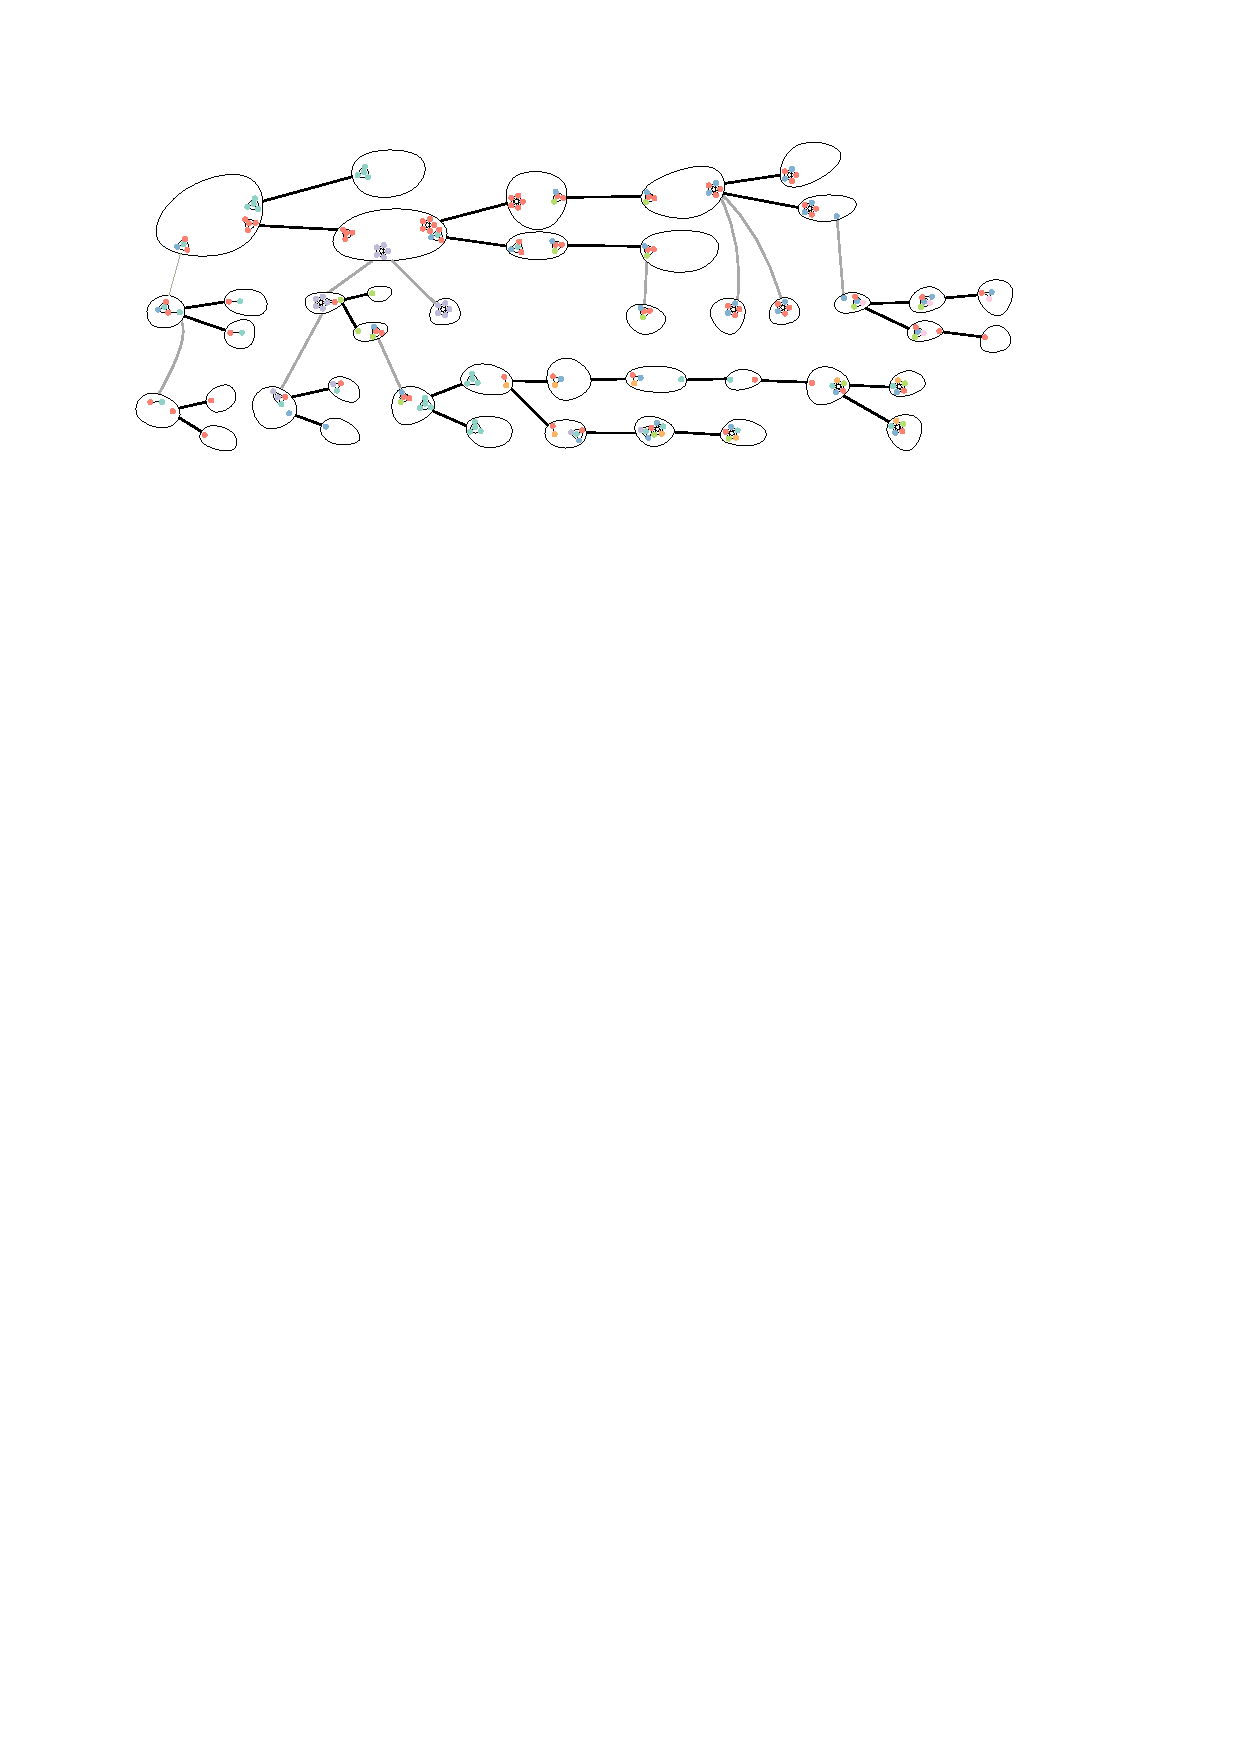
\includegraphics[page=1,width=.9\textwidth]{figs/t_tprime.pdf}}%
    \only<2>{\includegraphics[page=2,width=.9\textwidth]{figs/t_tprime.pdf}}%
    \only<3>{\includegraphics[page=3,width=.9\textwidth]{figs/t_tprime.pdf}}%
    \only<4>{\includegraphics[page=4,width=.9\textwidth]{figs/t_tprime.pdf}}%
    \only<5>{\includegraphics[page=5,width=.9\textwidth]{figs/t_tprime.pdf}}%
    \only<6>{\includegraphics[page=6,width=.9\textwidth]{figs/t_tprime.pdf}}%
  \end{center}

\end{frame}


\begin{frame}
  \frametitle{Tree decompositions}

  $\calT=(B_x:x\in V(T))$\\[1ex]

  \begin{center}
    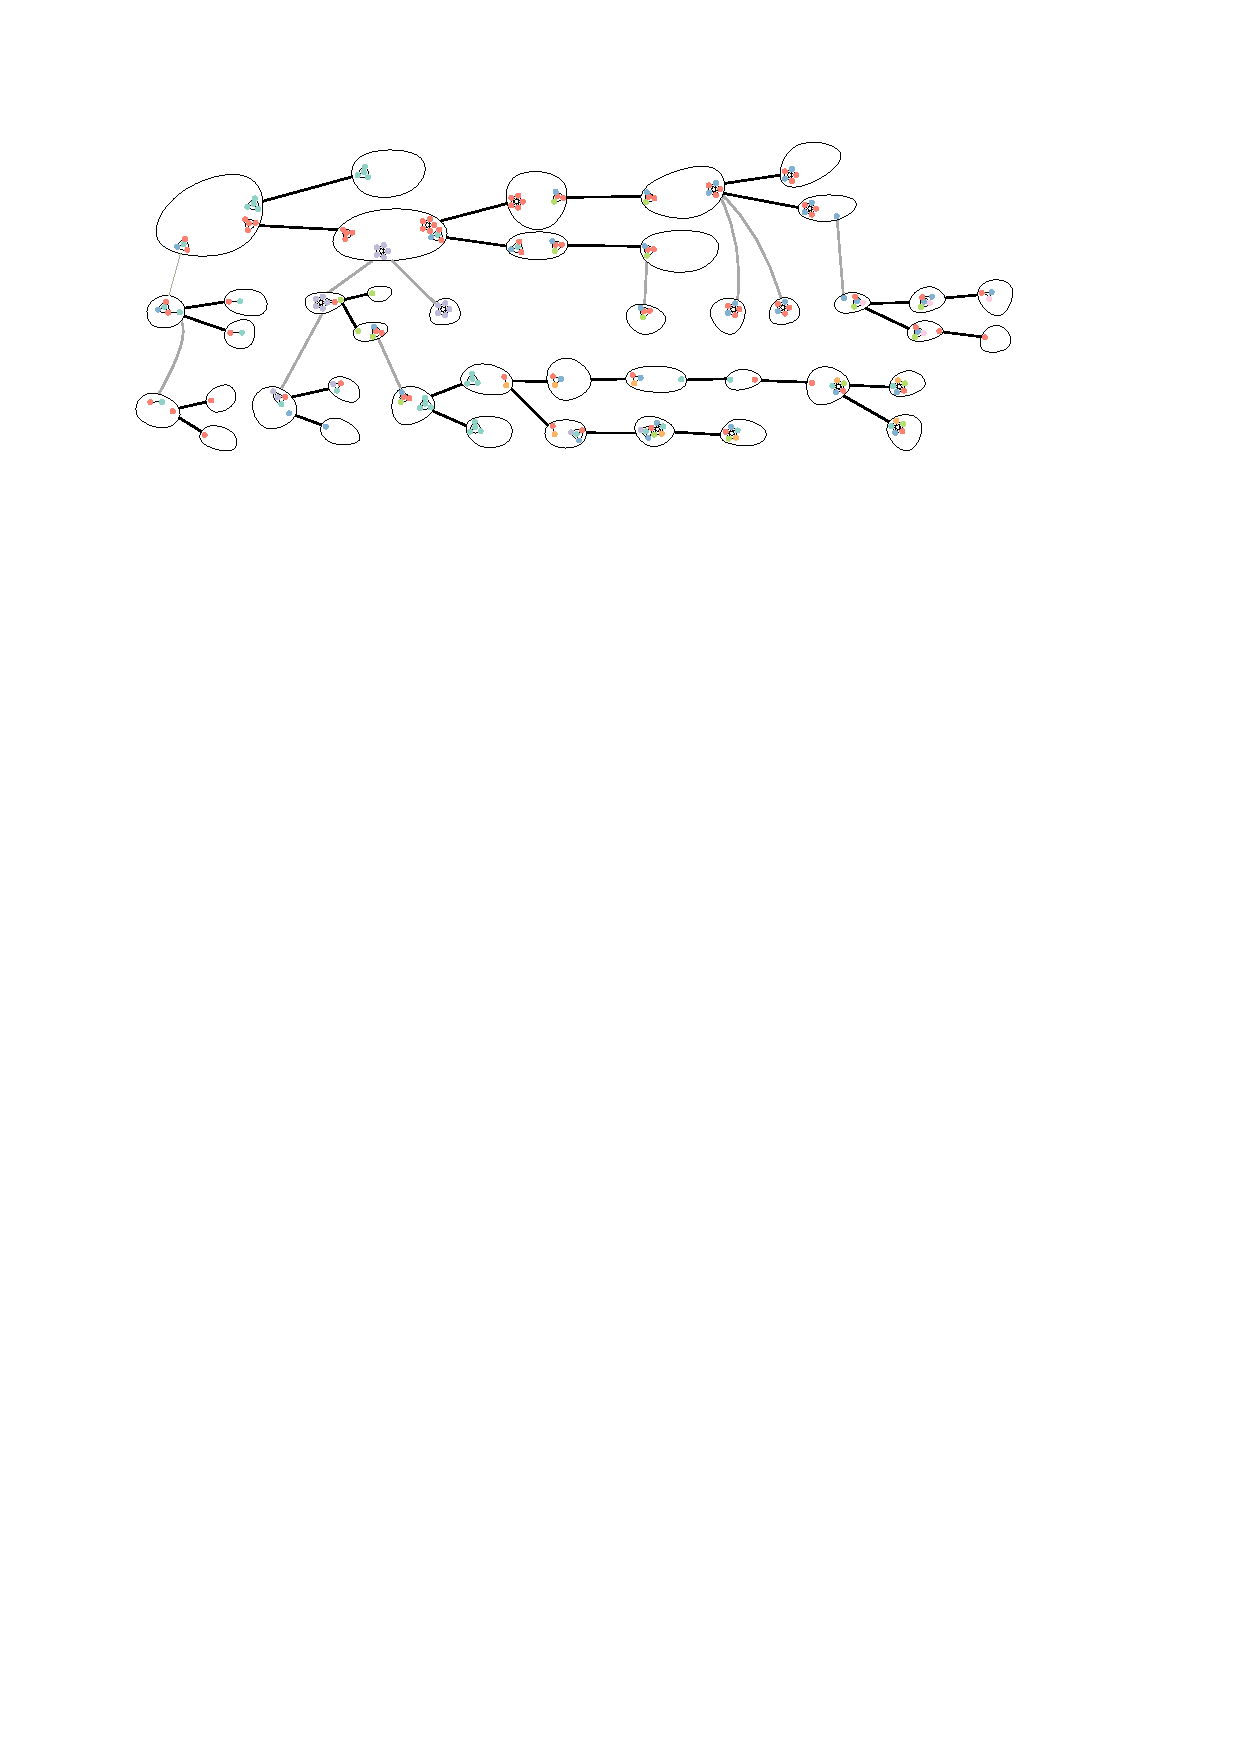
\includegraphics[page=1,width=.9\textwidth]{figs/t_tprime}
  \end{center}

  \emph{induced subgraph} $G[B_x]$ versus \emph{torso} $\torso{G}{B_x}$
  % $G$ versus $G^\star=\bigcup_{x\in V(T)}\torso{G}{B_x}$

\end{frame}

\begin{frame}
  \frametitle{Mixed Labelling Schemes}
  \framesubtitle{A First Try}

  \begin{itemize}
    \item Adjacency tester $A:(\{0,1\}^*)^2\to\{0,1\}$
    \item Identity tester $I:(\{0,1\}^*)^3\to\{0,1\}$
    \item Two graphs: $G^+$ and spanning subgraph $G$
    \item Label vertices \emph{and cliques} of $G^+$: $\mu:V(G)\cup K(G^+)\to\{0,1\}^*$
    \item $A(\mu(v),\mu(w))$ tests if $vw\in E(G)$
    \item Assign each vertex $u$ in a clique $K$ a (short) \emph{local identifier} $\kappa(K,u)$
    \item $I(\mu(K),\kappa(K,u),\mu(v))$ tests if $u=v$
  \end{itemize}
\end{frame}

\begin{frame}
  \frametitle{Mixed Labelling Schemes}
  \framesubtitle{Example Application}

  \begin{center}
    \only<+>{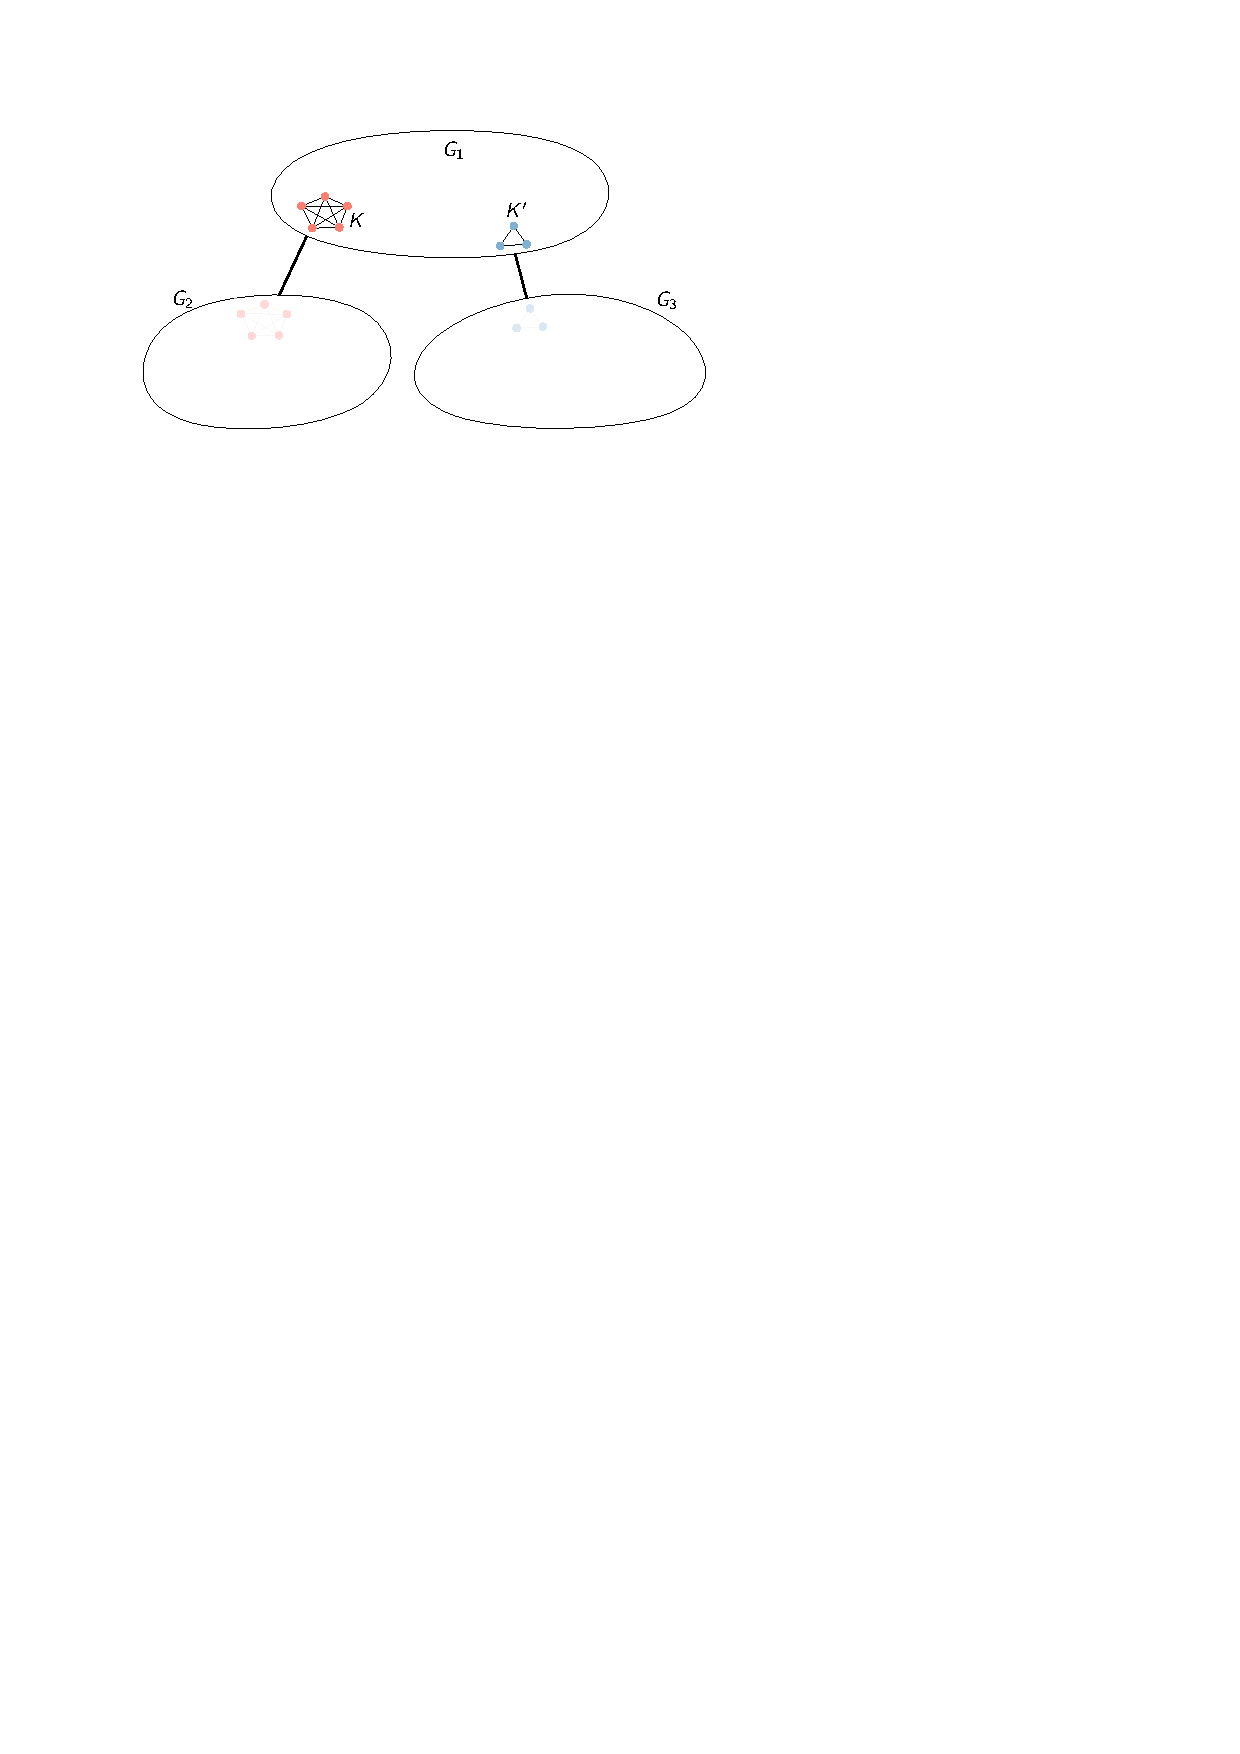
\includegraphics[page=1,width=\textwidth]{figs/mixed}}%
    \only<+>{\includegraphics[page=2,width=\textwidth]{figs/mixed}}%
    \only<+>{\includegraphics[page=3,width=\textwidth]{figs/mixed}}%
    \only<+>{\includegraphics[page=4,width=\textwidth]{figs/mixed}}%
    \only<+>{\includegraphics[page=5,width=\textwidth]{figs/mixed}}%
    \only<+>{\includegraphics[page=6,width=\textwidth]{figs/mixed}}%
    \only<+>{\includegraphics[page=7,width=\textwidth]{figs/mixed}}%
    \only<+>{\includegraphics[page=8,width=\textwidth]{figs/mixed}}%
    \only<+>{\includegraphics[page=9,width=\textwidth]{figs/mixed}}%
  \end{center}
\end{frame}


\begin{frame}
  \frametitle{Weighted Mixed Labelling Schemes}
  % \framesubtitle{A First Try}

  \begin{itemize}
    \item Adjacency tester $A:(\{0,1\}^*)^2\to\{0,1\}$
    \item Identity tester $I:(\{0,1\}^*)^3\to\{0,1\}$
    \item Two graphs: $G^+$ and spanning subgraph $G$
    \item Label vertices \emph{and cliques} of $G^+$: $\mu:V(G)\cup K(G^+)\to\{0,1\}^*$
    \item $A(\mu(v),\mu(w))$ tests if $vw\in E(G)$
    \item Assign each vertex $u$ in a clique $K$ a (short) \emph{local identifier} $\kappa(K,v)$
    \item $I(\mu(K),\kappa(K,u),\mu(v))$ tests if $u=v$\\[3ex]

    \item Weight function $\omega:V(G)\to\mathbb{R}^+$
    \item $|\mu(v)|\le\log(\omega(G)/\omega(v))+g_1(n)=\log \omega(G)-\log\omega(v) + g_1(n)$
    \item $|\kappa(K,u)|\le g_2(n)$
    \item $|\mu(K)|\le\log \omega(G)-\log\min_{u\in K}\omega(u) + g_3(n)$
    \item If $g_1,g_2,g_3\in o(\log n)$ then scheme is \emph{efficient}
  \end{itemize}
\end{frame}


\begin{frame}
  \frametitle{Weighted Mixed Labelling Schemes}
  \framesubtitle{Example Application}

  \begin{center}
    % \only<+>{\includegraphics[page=9,width=\textwidth]{figs/mixed}}%
    \only<+>{\includegraphics[page=10,width=\textwidth]{figs/mixed}}%
  \end{center}
\end{frame}

\begin{frame}
  \frametitle{GMST: Mixed Labelling Version}

  % A weighted $(g_1,g_2,g_3)$ mixed labelling scheme is \emph{efficient} if $g_1,g_2,g_3\in o(\log n)$.\\[2ex]

  \textbf{Theorem:}  For every graph $H$, every $H$-minor-free graph $G$ has a tree-decomposition whose torsos admit efficient weighted mixed labelling schemes.

  ($G^+=\torso{G}{B_x}$ is a torso, $G=G[B_x]$ is the spanning subgraph)

  \begin{center}
    \only<1>{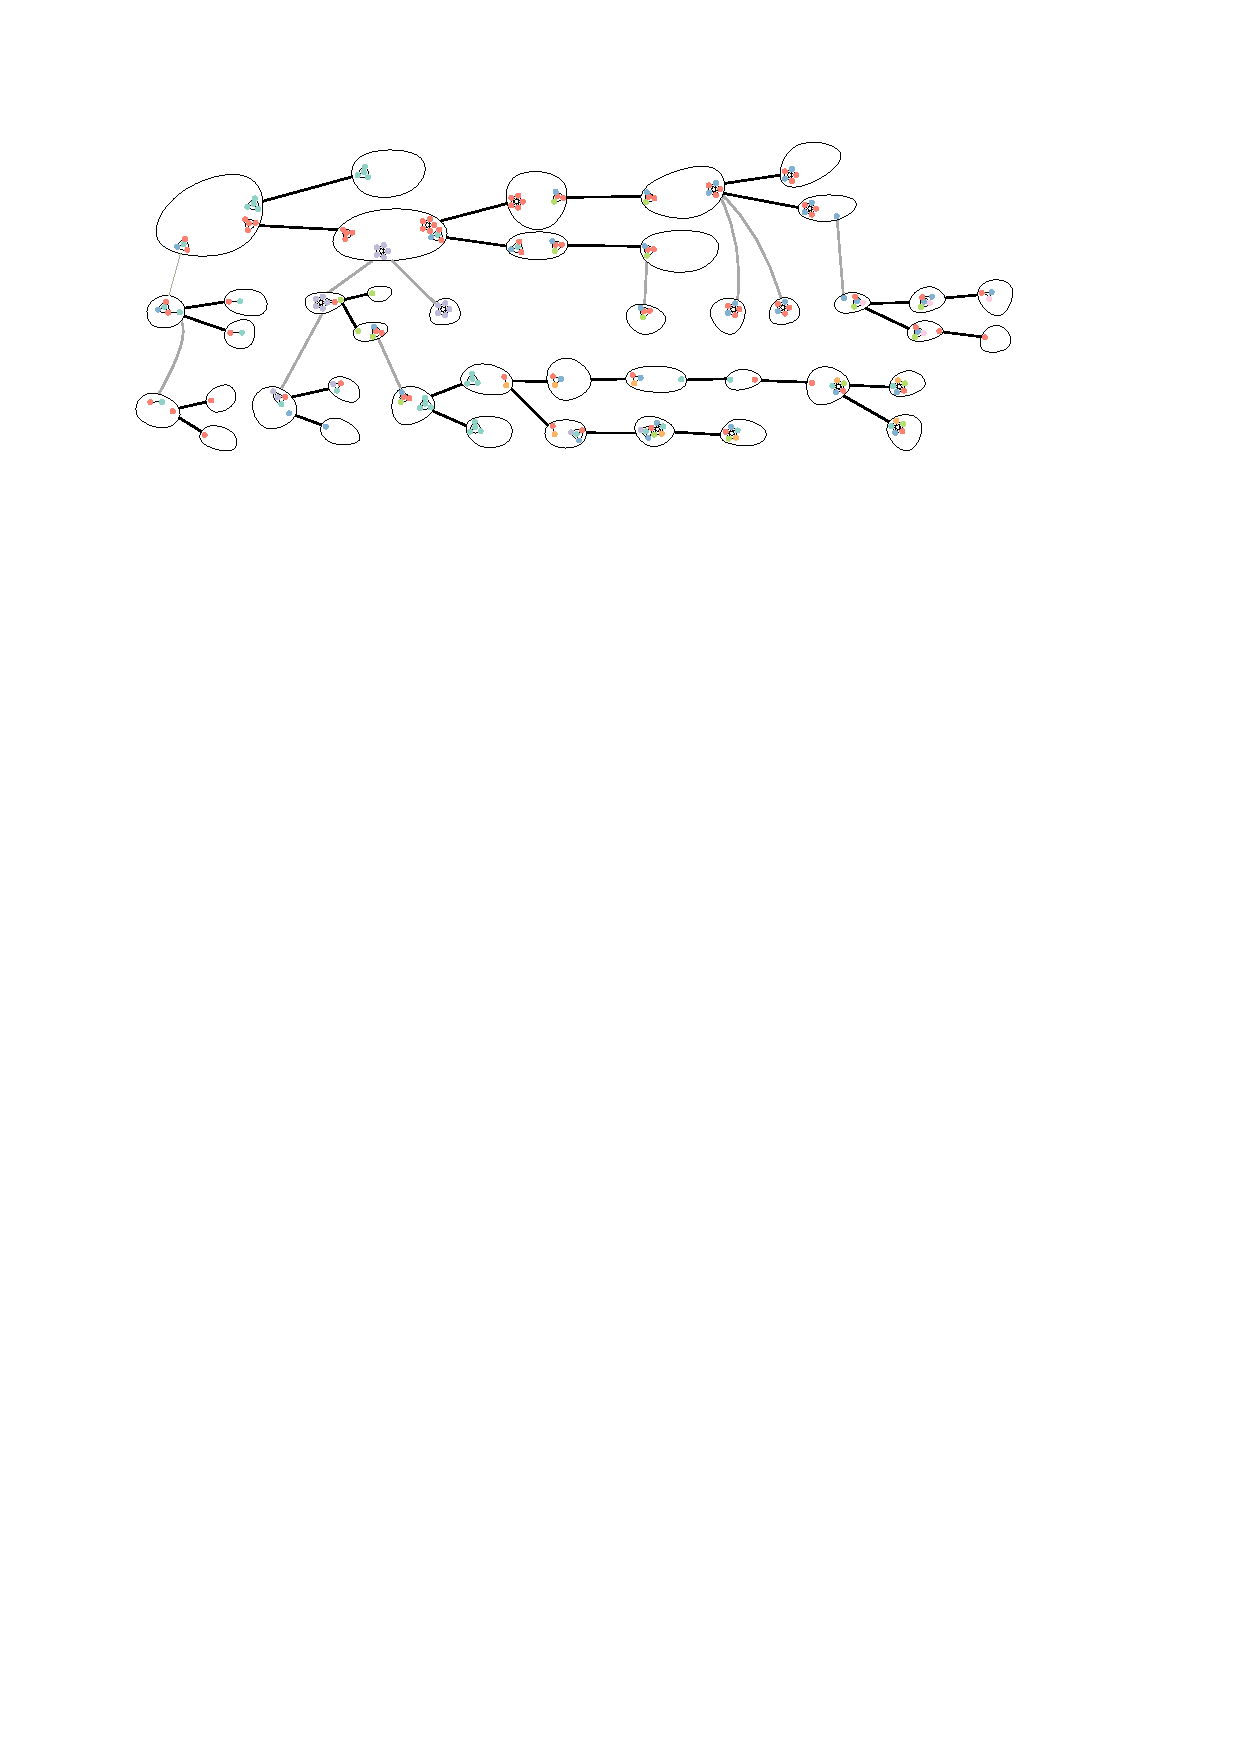
\includegraphics[width=.9\textwidth]{figs/t_tprime}}
    \only<2->{\includegraphics[page=7,width=.9\textwidth]{figs/t_tprime}}
  \end{center}
  \uncover<3->{Does this actually work?} \uncover<4->{\textbf{NO}}
\end{frame}

\begin{frame}
  \frametitle{Graphs with Short Tree Decompositions}
  \textbf{Theorem:} If each $n$-vertex $G\in\calG$ has a tree-decomposition of height $h=h(n)$ whose torsos come from a graph class $\calG'$ that has a weighted $(g_1,g_2,g_3)$ mixed labelling scheme, then $\calG$ has an $f(n)$-bit adjacency labelling scheme with $f(n)=\log n + \mathcolor{red}{h(n)\cdot g_3(n)} + o(\log n)$

\begin{center}
  % \only<1>{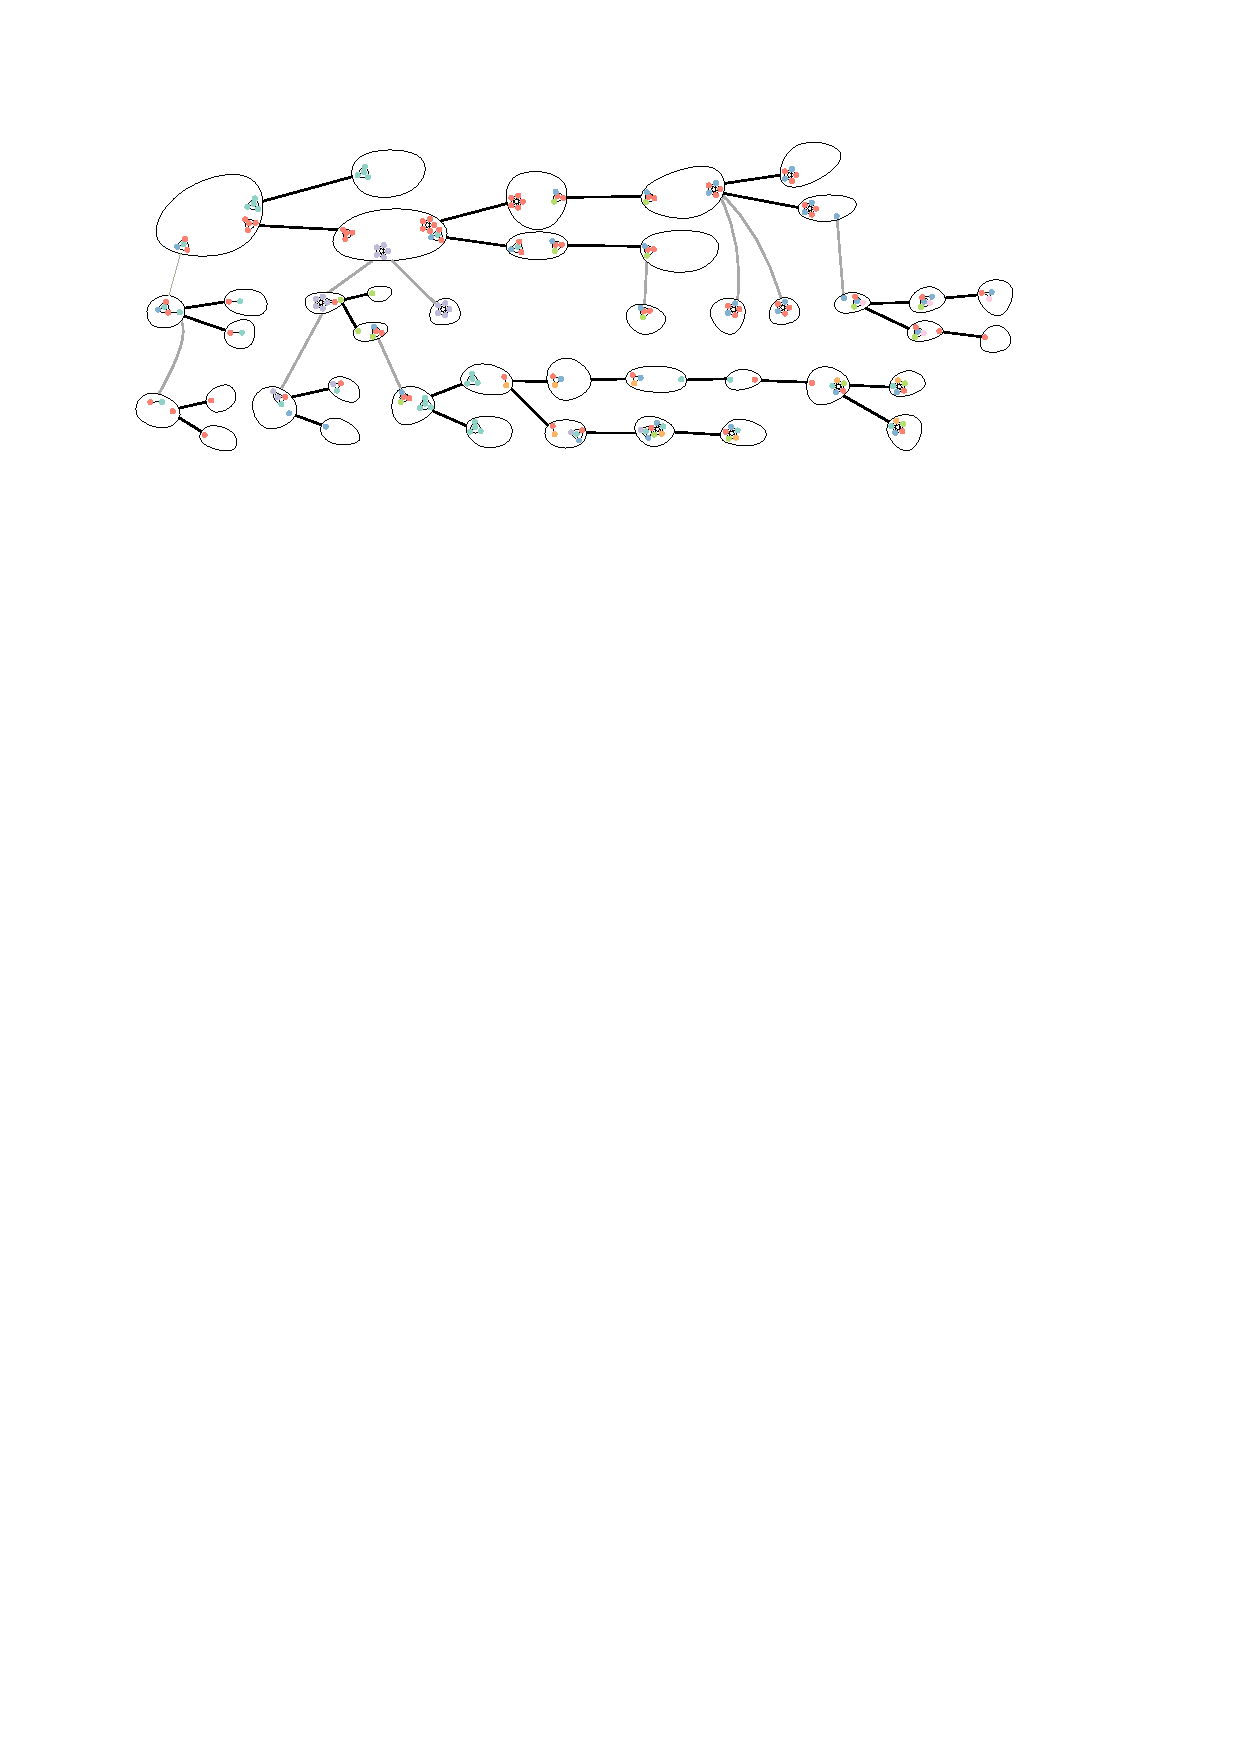
\includegraphics[width=.9\textwidth]{figs/t_tprime}}
  \includegraphics[page=7,width=.9\textwidth]{figs/t_tprime}
\end{center}
\end{frame}

\begin{frame}
  \frametitle{Decomposition into Skinny Subtrees}
  \begin{center}
    \only<1>{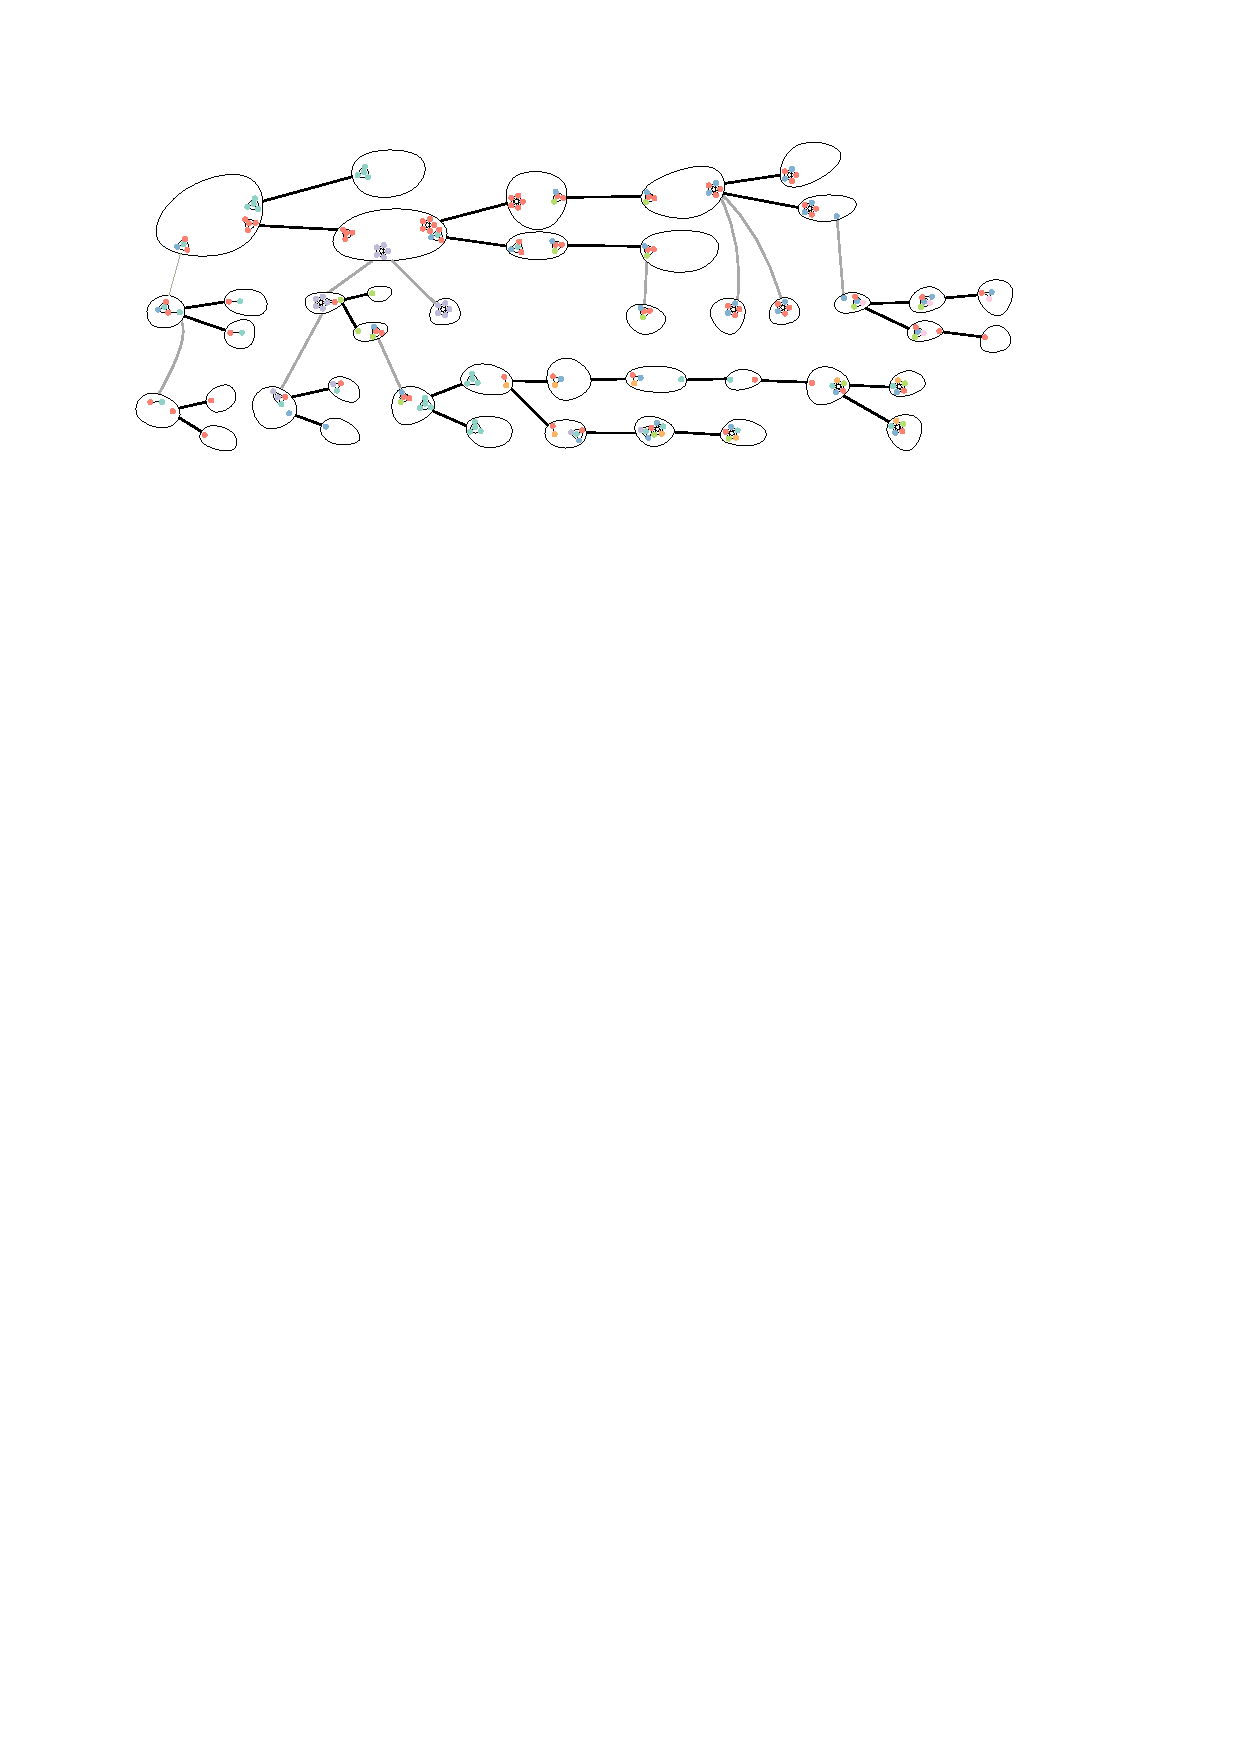
\includegraphics[page=1,width=.9\textwidth]{figs/t_tprime.pdf}}%
    \only<2>{\includegraphics[page=8,width=.9\textwidth]{figs/t_tprime.pdf}}%
    % \only<3>{\includegraphics[page=3,width=.9\textwidth]{figs/t_tprime.pdf}}%
    % \only<4>{\includegraphics[page=4,width=.9\textwidth]{figs/t_tprime.pdf}}%
    % \only<5>{\includegraphics[page=5,width=.9\textwidth]{figs/t_tprime.pdf}}%
    \only<3->{\includegraphics[page=6,width=.9\textwidth]{figs/t_tprime.pdf}}%
  \end{center}
  \uncover<1->{Choose $x$ if $|\bigcup_{y\in V(T_x)}B_y|>n/b$} \\
  \uncover<4->{Can get $h(n)=\log_b n$ by partitioning into $b$-skinny subtrees} \\
  \uncover<5->{Even for enormous $b$ (we use $b=2^{(\log n)^{3/4}}$, so $h=(\log n)^{1/4}$)}\\
  \uncover<6->{We just need a weighted mixed labelling scheme for $b$-skinny subtrees!}
\end{frame}

\begin{frame}
  \frametitle{Graphs with Skinny Tree-Decompositions}

  \textbf{Theorem:} If each $G\in\calG$ has a $b$-skinny tree-decomposition whose torsos are in a class $\calG'$ that has a weighted $(g_1,g_2,g_3)$ mixed labelling scheme then $\calG$ has a weighted $(g_1',g_2',g_3')$ mixed labelling scheme with \newline $g_i'(n)=g_i(n)+O(\log\log n + \log b)$.\\[1ex]

  \begin{center}
    \only<+>{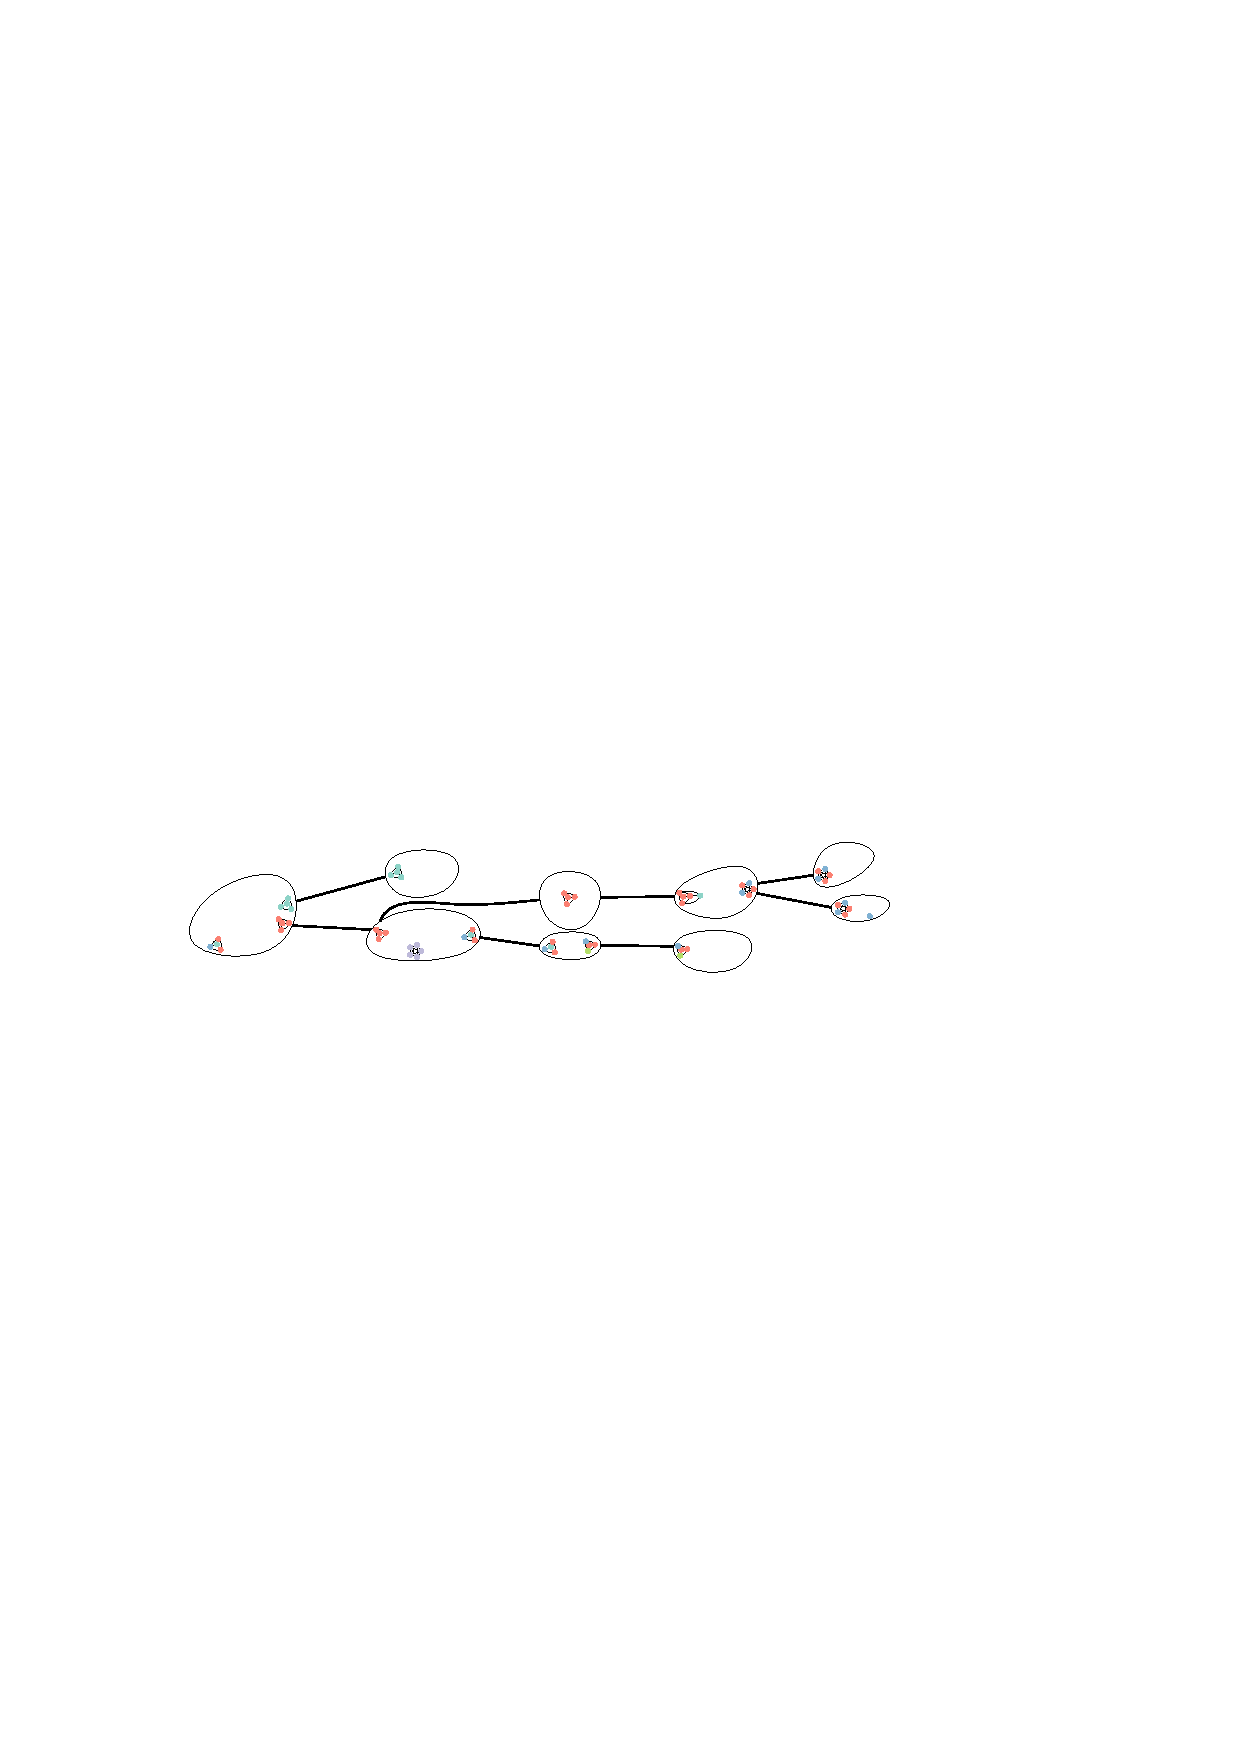
\includegraphics[page=1,width=.9\textwidth]{figs/skinny}}%
    \only<+>{\includegraphics[page=2,width=.9\textwidth]{figs/skinny}}%
    \only<+>{\includegraphics[page=3,width=.9\textwidth]{figs/skinny}}%
    \only<+>{\includegraphics[page=4,width=.9\textwidth]{figs/skinny}}%
    \only<+>{\includegraphics[page=5,width=.9\textwidth]{figs/skinny}}%
    \only<+>{\includegraphics[page=6,width=.9\textwidth]{figs/skinny}}%
    \only<+>{\includegraphics[page=7,width=.9\textwidth]{figs/skinny}}%
    \only<+>{\includegraphics[page=8,width=.9\textwidth]{figs/skinny}}%
    \only<+>{\includegraphics[page=9,width=.9\textwidth]{figs/skinny}}%
    \only<+>{\includegraphics[page=10,width=.9\textwidth]{figs/skinny}}%
    \only<+>{\includegraphics[page=11,width=.9\textwidth]{figs/skinny}}%
    \only<+>{\includegraphics[page=12,width=.9\textwidth]{figs/skinny}}%
    \only<+>{\includegraphics[page=13,width=.9\textwidth]{figs/skinny}}%
    \only<+>{\includegraphics[page=14,width=.9\textwidth]{figs/skinny}}%
    \only<+>{\includegraphics[page=15,width=.9\textwidth]{figs/skinny}}%
  \end{center}
\end{frame}


\begin{frame}
  \frametitle{Review}


  \textbf{Theorem:} If each $G\in\calG$ has a tree-decomposition whose torsos are in a class $\calG'$ that has an efficient mixed labelling scheme then $\calG$ has an efficient mixed labelling scheme.\\[1ex]

  \textit{Proof:} Take the tree decomposition of $G$ and turn it into a decomposition of height $\log_b n$ whose torsos have $b$-skinny tree decompositions.\hfill{QED}
  \\[2ex]

  \uncover<2->{To prove main result, use:\\
  \textbf{Theorem:}  For every graph $H$, every $H$-minor-free graph $G$ has a tree-decomposition whose torsos admit efficient weighted mixed labelling schemes.}

  \uncover<3->{Proof follows from techniques in [DEGJMM21]}

\end{frame}

\begin{frame}
  \frametitle{Summary/Conclusion}

  \begin{itemize}
    \item $(1+o(1))\log n$-bit adjacency labelling scheme for $H$-minor-free graphs
    \begin{itemize}
      \item weighted mixed labelling scheme
      \item solution for graphs with short tree decompositions
      \item solution for graphs with skinny tree decompositions
      \item partition of any tree decomposition into skinny subtrees whose contraction gives a short tree
    \end{itemize}
    \item Proof is constructive
    \begin{itemize}
      \item Polynomial time algorithm for computing the labelling
      \item $O((\log n)^{1/4})$-time adjacency testing procedure
    \end{itemize}
  \end{itemize}
  \begin{center}
    \uncover<2->{\Huge Thank You!}
  \end{center}
\end{frame}


\end{document}
